\section{Implementation of Core Functionalities}

\subsection{Operator}

\begin{figure}[H]
    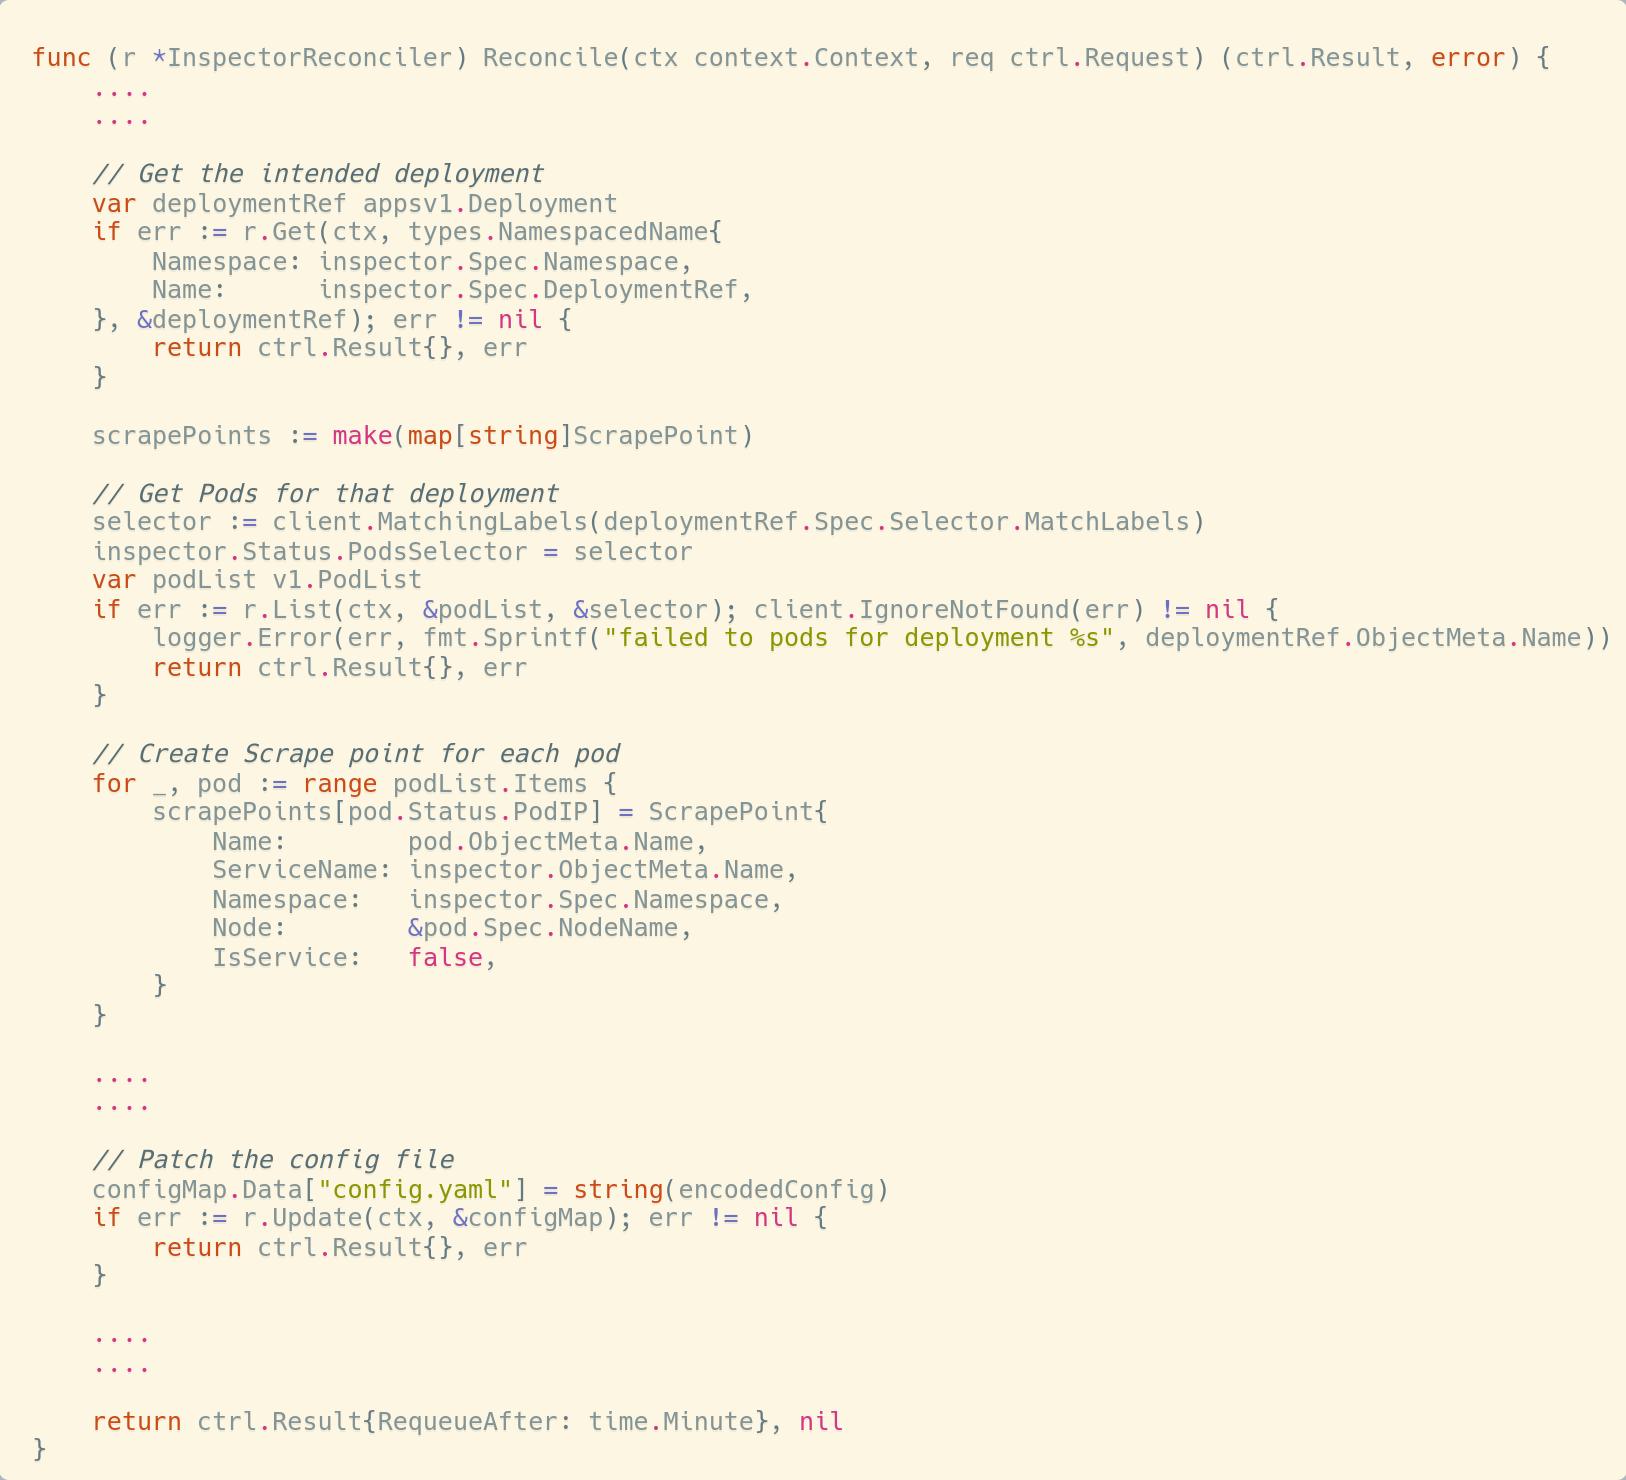
\includegraphics[width=14cm]{assets/implementation/reconcile-loop.png}
    \caption{Operator Reconciliation Loop (self-composed)}
    \label{fig:reconcile-loop}
\end{figure}

\subsection{Gazer}

\begin{figure}[H]
    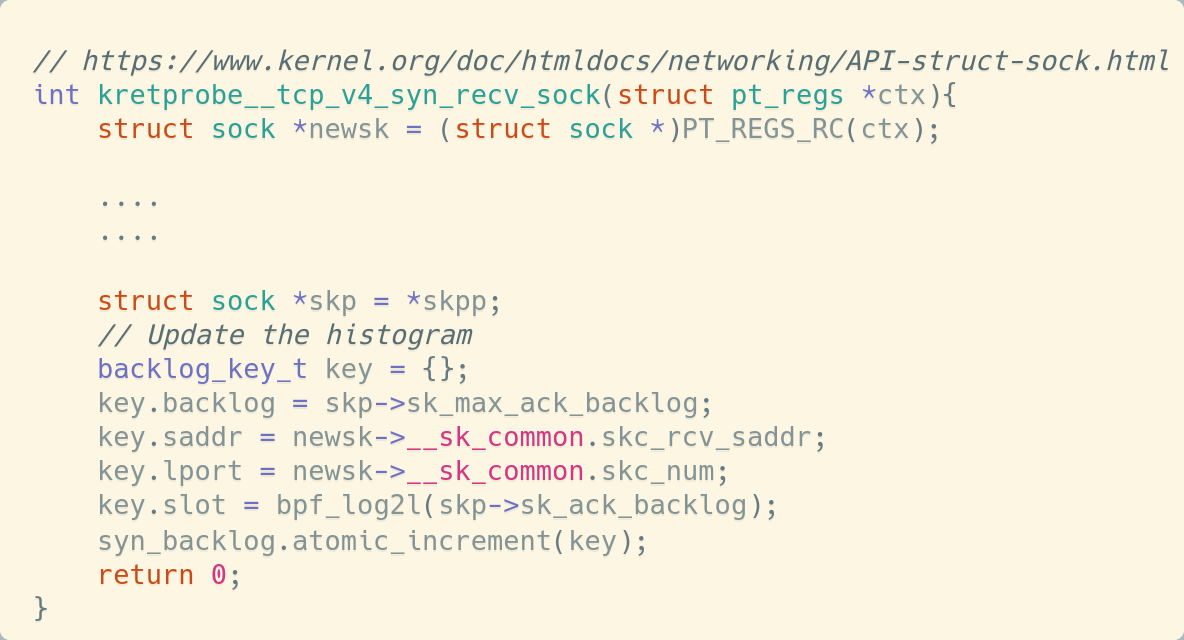
\includegraphics[width=14cm]{assets/implementation/backlog-probe.png}
    \caption{\ac{ebpf} probe to collecting tcp backlog (self-composed)}
    \label{fig:backlog-probe}
\end{figure}

\subsection{Sherlock}

\begin{figure}[H]
    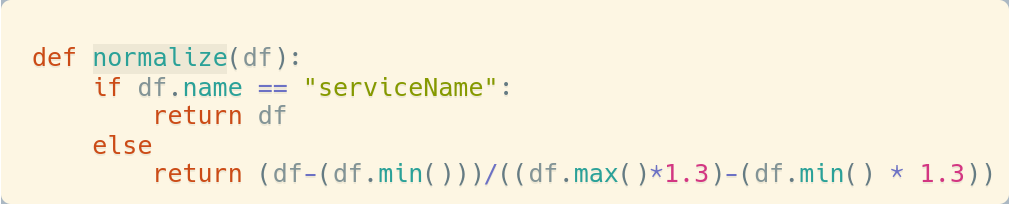
\includegraphics[width=14cm]{assets/implementation/normalize-data.png}
    \caption{Data normalization function (self-composed)}
    \label{fig:normalize-data}
\end{figure}


\begin{figure}[H]
    \centering
    \begin{subfigure}[b]{0.48\textwidth}
        \centering
        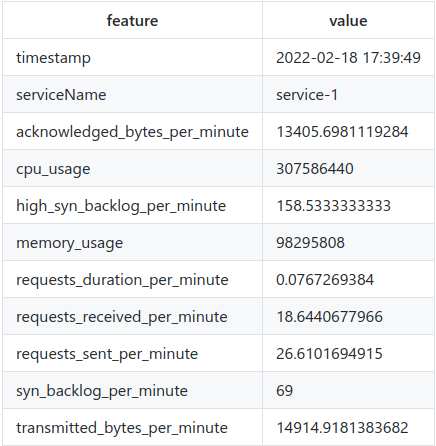
\includegraphics[width=\textwidth]{assets/implementation/before-normalization.png}
        \caption{Before Normalization}
        \label{fig:before-normalization}
    \end{subfigure}
    \hfill
    \begin{subfigure}[b]{0.49\textwidth}
        \centering
        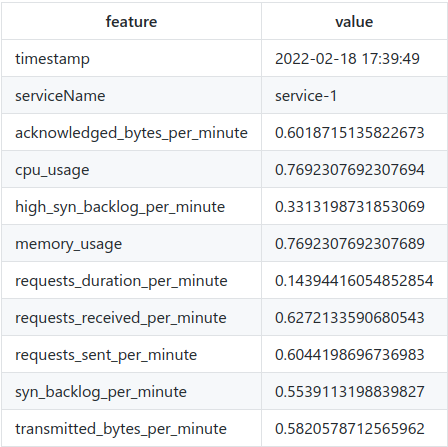
\includegraphics[width=\textwidth]{assets/implementation/after-normalization.png}
        \caption{After Normalization}
        \label{fig:after-normalization}
    \end{subfigure}
    \hfill
       \caption{Comparsion of a data point before and after normalization (self-composed)}
\end{figure}

\begin{figure}[H]
    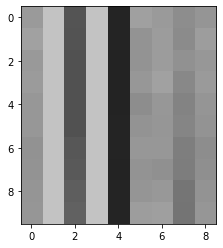
\includegraphics[width=7cm]{assets/implementation/visualize-representation.png}
    \caption{Visualization of encoded time series (self-composed)}
    \label{fig:visualize-representation}
\end{figure}
